\section{The weighted kernel under the triangular degree cutoff}\label{sec:carrier}

Fix $\lambda$ as in Theorem~\ref{th:rank} and one block. Let $C=1-\kappa g$. Over $\mathbb F=\RR(\kappa)$ there are two immediate sources of zero periods. A form $C\nu$ cancels the multiplier in the denominator, so any unweighted relation $\nu$ gives a weighted one. A multiple of $\Omega$ vanishes on the tangent to every oval. To identify the rank we must show that these sources exhaust the kernel \emph{within the prescribed degree}. Write $\mathcal T(X)$ for the span of $T_a(x)T_b(y)$ in the block with $a+b\le X$ and $b<M$.

A relative exactness criterion for generic Darboux centers was described by Christopher and Marde\v{s}i\'c in conference lectures~\cite{relative}. It assumes normal crossings with the line at infinity and irrational ratios of residues on distinct components. In our grid the parallel lines in one family meet at infinity and have equal residues. We work directly with the polynomial modes and their degree cutoff.

\begin{proposition}\label{prop:kernel}
Extending constant spaces to $\mathbb F$, the weighted kernel on $W(S)$ is the direct sum
\begin{equation}\label{eq:kernel}
 C\,\ker\bigl(\Lu|_{W(S-M)}\bigr)\ \oplus\ \mathcal T(S-N-M)\,\Omega .
\end{equation}
\end{proposition}

\subsection{What the moments determine}
The Taylor coefficients of $L_C$ at $h=0$ belong to $\mathbb F$. In the coordinates \eqref{eq:morse} the new factor is $(1-\kappa e_l e^{-v^2/2})^{-1}$. Writing \(q=e_l\kappa\), we have the germ
\[
 \frac{1}{1-qe^{-v^2/2}}=\frac{1}{1-q}
   \sum_{j\ge0}\left(\frac{q}{1-q}\right)^j (e^{-v^2/2}-1)^j .
\]
Only \(j\le n\) contribute to the coefficient of \(v^{2n}\), whose denominator therefore divides \((1-q)^{n+1}\). Differentiation in the Morse coordinate and multiplication by the unweighted analytic factors introduce no other parameter poles. Green's formula on the Morse ellipse therefore defines the period map into $\mathbb F[[h]]$. For each real $|\kappa|<1$ the germ converges, and analyticity in $h>0$ identifies its kernel with that of the actual integrals.

Clear denominators in a rational kernel element and write $\omega(\kappa)=\sum_{m=0}^d\kappa^m\omega_m$. Its Taylor rows vanish identically in $\kappa$, so its period is zero for all real $|\kappa|<1$ and $h>0$. Put
\[
 B=\sum_{m=0}^d g^{d-m}\omega_m .
\]
For fixed $h>0$, use $\tau=e_l\kappa$ on its oval. The uniformly convergent geometric series for $(1-\tau\cos\eta)^{-1}$ gives, at degree $d+n$ in $\tau$, the numerator
\[
 (\cos\eta)^n\sum_{m=0}^d e_l^m(\cos\eta)^{d-m}\omega_m
       = e_l^d(\cos\eta)^n B .
\]
Thus $\oint_{\gamma_h}(\cos\eta)^n B/|fg|=0$ for every $n\ge0$. Multiplication by $g=T_M$ preserves the block, since its shifts on the vertical sine and cosine indices are $b\mapsto |b\pm M|$. Consequently the \emph{full} angle pullback $F\,d\xi+G\,d\eta$ of $B/|fg|$ is odd under pullback by each reflection, by \eqref{eq:angles}. On this diagonal block the four oriented quadrant integrals agree. In particular $F(\xi,0)=G(0,\eta)=0$.

In the positive quadrant put $y_0=e^{-h}$ and $u=\cos\eta$. Then $y_0<u<1$, $\cos\xi=(y_0/u)^{1/\lambda}$. In the counterclockwise direction $u$ decreases. Reversing the integration limits gives
\begin{equation}\label{eq:moment}
 \int_{y_0}^1 u^n\left(-\frac{F}{\lambda u\tan\xi}
                      +\frac{G}{\sin\eta}\right)\dd u=0 .
\end{equation}
For fixed $h>0$ the arc and its endpoints lie inside the angle square. At $u\uparrow1$, $\tan\xi$ has a positive finite limit, $F=O(\sqrt{1-u})$, and $G/\sin\eta=O((1-u)^{-1/2})$. This last term can be unbounded. At $u\downarrow y_0$, $\tan\xi\asymp\sqrt{u-y_0}$ and $\sin\eta$ has a positive limit. The first term is $O((u-y_0)^{-1/2})$ and the second is $O(\sqrt{u-y_0})$. The bracket is integrable at both ends and continuous in the interior. Polynomial density in $C[y_0,1]$ implies that its signed measure is zero, hence that the bracket vanishes at every interior point. As $h$ varies, this says that $B$ vanishes on the oval tangents throughout the quadrant. Thus $B\wedge\Omega$ is a polynomial two-form vanishing on an open set, so it is identically zero.

The coefficients $\lambda f'g$ and $fg'$ are coprime in $\RR[x,y]$. Indeed $f,g$ have only simple roots and factors in separate variables are relatively prime. Unique factorization gives $B=B_0\Omega$ with polynomial $B_0$.

\subsection{Polynomial division and the terms above the degree cutoff}
Modulo \(C\) one has \(\kappa g\equiv1\), hence \(\omega(\kappa)\equiv\kappa^d B\). Divide \(\kappa^d B_0\) by \(C\) in \(\mathbb F[x][y]\). The divisor \(C\) has leading \(y\)-coefficient \(-2^{M-1}\kappa\). Starting with the polynomial numerator already cleared above, long division introduces only powers of \(\kappa\) in parameter denominators. These are invertible for \(0<\kappa<1/2\). It follows that
\begin{equation}\label{eq:division}
 \omega=C\nu+R\Omega,\qquad \deg_yR<M .
\end{equation}
We may take both $R$ and $\nu$ in the chosen frequency classes. To see this, expand scalars in $T_aT_b$, and the $dy,dx$ coefficients in the respective bases of \eqref{eq:modes}, allowing the free cosine index to be zero. Project each expansion to the block. The indices in $\A_k$ obey $a\equiv N/2^k\pmod{2N/2^k}$, and similarly for $\B_l$. Modulo \(2N/2^k\), the class \(N/2^k\) equals its negative, and \(N\) is a multiple of this modulus since \(k\ge1\). Thus \(a\mapsto|a\pm N|\) preserves membership and its complement. The same holds for \(b\mapsto|b\pm M|\). Products with $C$ and products of a scalar with $\Omega$ have precisely these folded shifts, by the sine and cosine products. The cosine index zero stays outside even when shifted to $N$ or $M$, and a zero sine is simply zero. This proves that the projections commute with the products in \eqref{eq:division}. The projection preserves the bound on $\deg_yR$.

For $A_{ab}=T_a(x)T_b(y)$ with $0<b<M$, set
\begin{equation}\label{eq:delta}
 D_\lambda A_{ab}=\lambda f'T_aT_b\,dx + M f T_a U_{b-1}\,dy .
\end{equation}
Here $T_a$ is evaluated at $x$, and $T_b$ and $U_{b-1}$ at $y$. The identity $T_b U_{M-1}=U_{M-b-1}+gU_{b-1}$ gives the actual quotient and remainder of $A_{ab}\Omega$ on division by $C$, namely
\begin{align}
 A_{ab}\Omega &=-\kappa^{-1}C D_\lambda A_{ab} + E(A_{ab}),\nonumber\\
 E(A_{ab})&=\kappa^{-1}\lambda f'T_aT_b\,dx+
 M f T_a\bigl(U_{M-b-1}+\kappa^{-1}U_{b-1}\bigr)\,dy .
 \label{eq:rem}
\end{align}
Both components of $E(A_{ab})$ have vertical degree below $M$. Thus $\widehat\nu=\nu-\kappa^{-1}D_\lambda R$ and $E(R)$ are the quotient and remainder of $\omega$. Per coefficient of $x^j$, univariate division by $C\in\mathbb F[y]$ lowers the degree of the quotient by at least $M$ and does not raise the degree of the remainder. Hence $\widehat\nu\in W(S-M)$, and from the $dx$ remainder $\lambda f'R/\kappa$ we get $\deg R\le S-N$.

The possible excess over the second summand in \eqref{eq:kernel} is supported on
\begin{equation}\label{eq:shell}
 \mathcal H=\{(a,b)\in\A_k\times\B_l: b<M,\quad S-N-M<a+b\le S-N\}.
\end{equation}
Decompose $R=R_{\rm low}+R_{\rm high}$ at this cutoff. Then $D_\lambda R_{\rm low}\in W(S-M)$ by \eqref{eq:delta}. Since $L_C[\omega]=\Lu[\nu]$, a nonzero $R_{\rm high}$ would yield a relation of the unweighted periods of $V(S-M)$ and of the forms $D_\lambda A_{ab}$ for $(a,b)\in\mathcal H$. Here $V(S-M)$ can replace $W(S-M)$ by its spanning property. A nonzero finite Taylor minor preserves independence of real columns after extending scalars to $\mathbb F$.

\subsection{A shared pole and its separation}
In the block of odd indices for $N=M=4$, $S=12$, the pair $(3,3)\in\mathcal H$ contributes a term at $(7,3)$. The allowed unweighted form $E_{7,1}$ in $V(8)$ has exactly the same horizontal frequency. At a fixed anisotropy both reduced transforms have the horizontal pole $s=-3/(4\lambda)$. The vertical base classes $3/4$ and $1/4$ distinguish them. Figure~\ref{fig:rank} shows the auxiliary family used to test the four high terms. Here \(W(8)\) has dimension 20 and its unweighted rank is 14, so six relations can be multiplied by \(C\). Three allowed multiples of \(\Omega\) have \(a+b\le4\). Once the four high terms have been excluded, these give all nine relations on \(W(12)\).

\begin{figure}[tb]
\centering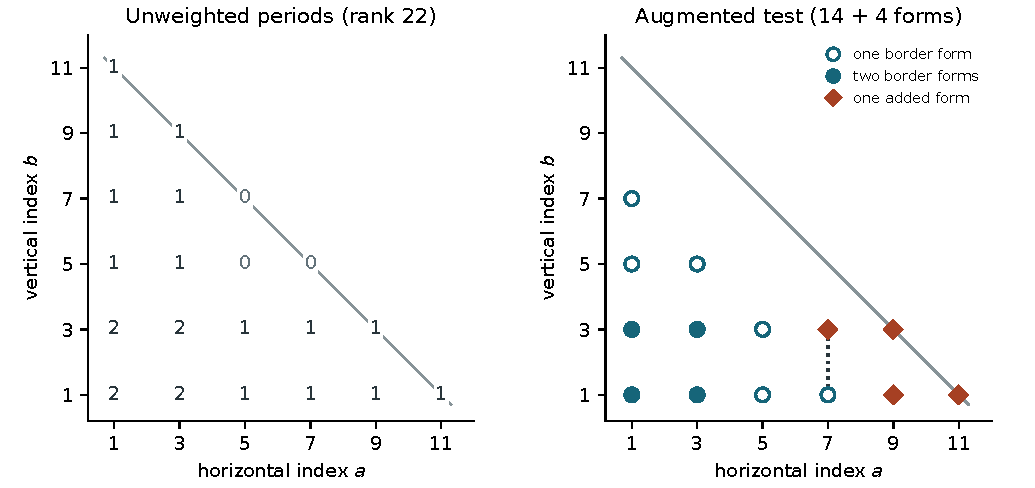
\includegraphics[width=.96\linewidth]{figures/frequencies.pdf}
\caption{Odd indices at \(N=M=4,\ D=11\). Left, the numbers count the \(E,F\) forms retained from the 42 original directions, giving unweighted rank 22. Right, six open and four filled circles represent the \(6+2\cdot4=14\) forms of \(V(8)\). Each diamond marks the upper index of one additional form \(D_\lambda A_{ab}\). The dotted segment joins two different vertical frequencies sharing horizontal index 7. Independence of these 18 forms rules out the high terms in the kernel. The full weighted rank is \(42-(6+3)=33\).}\label{fig:rank}
\end{figure}

\begin{lemma}\label{lem:shell}
The periods $\Lu[V(S-M)]$ together with $\Lu[D_\lambda A_{ab}]$ for $(a,b)\in\mathcal H$ are linearly independent at every transcendental $\lambda>1$.
\end{lemma}
\begin{proof}
Let the anisotropy vary as $t>1$. The sine and cosine products give the two horizontal indices $a+N, |a-N|$ in $D_t A_{ab}$. At the upper index the coefficients of $(E,F)$ are $(M/2,tN/2)$, and at the lower they are $(M/2,\sgn(N-a)tN/2)$. Since $a=N$ is excluded, both pairs are defined. Lemma~\ref{lem:lift} applies to this whole augmented list. In a putative polynomial relation write $q_{ab}(t)$ for the coefficient of $D_t A_{ab}$. Reduce by \eqref{eq:shift} and apply Lemma~\ref{lem:classes} to obtain a separate rational identity for \emph{each pair} of base frequencies. This step uses the open cone in $(z,w)$, including for the two summands of every $D_t A_{ab}$.

Fix a vertical index $b$ with some $q_{ab}\ne0$. Since $b<M$, it already specifies the base $v=b/M$. Among those coefficients at $b$, choose the largest horizontal index $a$. Write $A=1+a/N$, $z_0=1-A=-a/N$, and take the identity for the pair $(A_*,v)$. Consider the residue at $z=z_0$. Every ordinary term in $V(S-M)$ in this class has vertical index $b'\ge b$, hence horizontal index $a'\le S-M-b<a+N$ by the strict inequality in \eqref{eq:shell}. It cannot have this pole. Any other high term in this vertical class must have the same $b$, since all high vertical indices are below $M$. Its upper horizontal index is smaller than $a+N$, and every lower index $|a'-N|$ is strictly smaller as well. Formula \eqref{eq:shift} puts all their horizontal poles to the right of $z_0$.

The sole remaining upper term, after suppression of the common base factors, is
\[
 \sigma_{a+N,b}\,q_{ab}(z/w)\frac{z}{2w}
        \bigl[A(w-1)-v(z-1)\bigr] B_A(z) .
\]
Here $\sigma_{a+N,b}=\pm1$ is the phase of this shifted mode. For every fixed real $w>1$ all vertical rational factors are finite. The finite sum permits termwise residues, and \eqref{eq:shift} gives $\rho=\Res_{z=z_0}B_A(z)\ne0$. Its residue identity is
\begin{equation}\label{eq:residue}
 0=\sigma_{a+N,b}\,\rho\,q_{ab}(z_0/w)\frac{z_0}{2w} A(w-1+v),\qquad w>1 .
\end{equation}
All factors outside $q_{ab}$ are nonzero on this interval. As $z_0/w$ ranges over $(z_0,0)$ the polynomial $q_{ab}$ must vanish, a contradiction. Thus every high coefficient vanishes. Independence of $V(S-M)$ at a transcendental parameter then forces the remaining polynomial coefficients to vanish as well. This proves the lemma, including the case $\mathcal H=\varnothing$.
\end{proof}

\begin{proof}[Conclusion of Proposition~\ref{prop:kernel} and Theorem~\ref{th:rank}]
Lemma~\ref{lem:shell} gives $R_{\rm high}=0$. Equation \eqref{eq:division} now has $R\in\mathcal T(S-N-M)$ and $\nu\in W(S-M)$ with $\Lu[\nu]=0$. Conversely both summands in \eqref{eq:kernel} have zero weighted period and degree at most $S-1$. Their intersection is zero, since the $dx$ component of $E(R)$ is $\lambda f'R/\kappa$, which vanishes only for $R=0$.

The first summand has dimension $P(S-M-N)+P(S-2M)$ by \eqref{eq:pure}. The second has dimension $P(S-N-M)-P(S-N-2M)$ by shifting $b$ by $M$. Subtracting their sum from $2P(S)$ gives \eqref{eq:carrier}. A maximal nonzero Taylor minor over $\mathbb F$ is a rational function whose denominator has no zero in $(0,1/2)$ and whose numerator has finitely many roots. Larger minors vanish identically. At every real parameter avoiding these roots the actual germs therefore have the calculated rank. Take the union of the exceptional sets for the finitely many blocks. The two summands of~\eqref{eq:kernel} specialize into the real kernel, remain disjoint by~\eqref{eq:rem}, and have the required nullity there. For a fixed grid the complement contains rational \(\kappa\). One may even fix \(\lambda=\pi\) and one real \(\kappa\) for all integer budgets and grids, since the union of their finite exceptional sets is countable.
\end{proof}
